The kinematic model is tested by a series of specific control signal. By pushing the control signal into the estimation model and comparing the output with the car behavior published by Mocap, the kinematic model can be verified. The result is shown in the figure \ref{fig:mesh1}.

\begin{figure}[h]
    \centering
    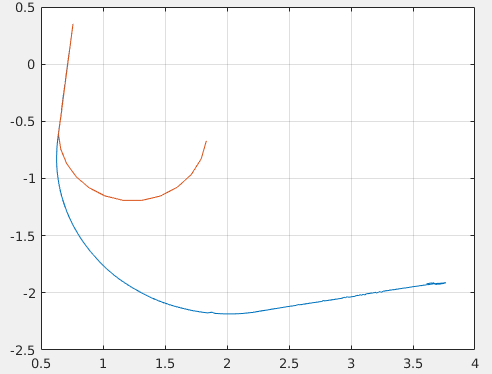
\includegraphics[width=0.85\textwidth]{./figures/kmver}
    \caption{Model and car behavior under a series of specific control signal}
    \label{fig:mesh1}
\end{figure}

As can be seen in the figure \ref{fig:mesh1}, red curve represents the model behavior while the blue one is the real car. The most probably reason that the deviation exists is that the car slips when turing.


\subsection{Dynamic model equations}

\begin{align*}
    & x_g(k+1) = x_g(k) + T_s (v_x(k) \cos(\psi(k)) - v_y(k) \sin(\psi(k)) \\
    & y_g(k+1) = y_g(k) + T_s (v_x(k) \sin(\psi(k)) + v_y(k) \cos(\psi(k)) \\
    & \psi(k+1) = \psi(k) + T_s r(k)\\
    & v_x(k+1) = v_x(k) + T_s / m C_f (\arctan((v_y(k)+r(k) l_f)/v_x(k)) - \delta(k)) \sin(\delta(k)) + T_s r(k) v_y(k)\\
    & v_y(k+1) = v_y(k) - T_s / m C_r \arctan((v_y(k)-r(k) l_r)/v_x(k)) - \\
    & \hspace{19mm}T_s C_f / m (\arctan((v_y(k)+r(k) l_f)/v_x(k))-\delta(k)) \cos(\delta(k)) - T_s r(k) v_x(k)\\
    & r(k+1) = r(k) - T_s l_f C_f/J_z \cos(\delta(k)) (\arctan((v_y(k)+r(k) l_f)/v_x(k))-\delta(k)) +\\
    & \hspace{19mm}T_s C_r / J_z \arctan((v_y(k)-r(k) l_r)/v_x(k))\\
    & v(k+1) = v(k) + T_s (v_ref(k) - \sqrt{v_x(k)^2 + v_y(k)^2})/\tau
\end{align*}

The $v_x,v_y$ are the velocity component at local coordinate, while $x_g, y_g$ are the position component at global coordinate.\\
There are three parameters in the model need to be defined i.e.  inertia of the car around z-direction $J_z$, cornering stiffness for front and rear wheels $C_f, C_r$. The estimation of these will be described next.

\subsection{Parameter estimation}

Here we use similar method to the one used in time-constant estimation. By putting certain series of input signals, both velocity and steering angle, the Mocap system generate the corresponding position signals as car running. Meanwhile in Matlab we generate the estimated position signals with the dynamic model given the same series of input.
The next step is to use Matlab
Will do it with Matlab function \texttt{Simulink Design Optimization} toolbox to find the optimize solutions of the problem in
\begin{equation}
  \min_{J_z, C_f, C_r} estimate\_error = (measurement - estimate\_position)^2
\end{equation}
The aim is to generate a qualified dynamic model which will be used as the inner model of the MPC controller, in order to drive the car as fast as possible. But due to the time limitation, we have not manage to achieve some satisfying parameters.
\end{document}
